\documentclass[border=2mm]{standalone}
\usepackage{pgfplots}
\pgfplotsset{compat=1.18}
\usetikzlibrary{arrows.meta, 
  calc, 
  positioning, 
  decorations.pathreplacing, 
  calligraphy}

\usepackage{xcolor}
\definecolor{den-1}{HTML}{111111}   % Đen #111111
\definecolor{den-2}{HTML}{222222}   % Đen #222222
\definecolor{den-3}{HTML}{333333}   % Đen #333333
\definecolor{den-4}{HTML}{444444}   % Đen #444444
\definecolor{den-5}{HTML}{555555}   % Đen #555555
\definecolor{den-6}{HTML}{666666}   % Đen #666666

\definecolor{do-1}{HTML}{440000}   % Đỏ #440000 trầm hơn, hợp với đen #111111
\definecolor{do-2}{HTML}{660000}   % Đỏ #660000 sẫm, hợp với đen #222222
\definecolor{do-3}{HTML}{880000}   % Đỏ #880000 đậm vừa, hợp với đen #333333
\definecolor{do-4}{HTML}{AA0000}   % Đỏ #AA0000 tươi vừa, hợp với đen #444444
\definecolor{do-5}{HTML}{CC0000}   % Đỏ #CC0000 tươi hơn, hợp với đen #555555
\definecolor{do-6}{HTML}{EE0000}   % Đỏ #EE0000 sáng hơn, hợp với đen #666666

% Thiết lập vị trí đặt nhãn gốc tọa độ
\tikzset{
  >=Stealth,
  originlabel/.style={
    font=\small\sf,
    anchor=north east, % Vị trí tương đối so với gốc
    yshift=-0.1ex,     % Điều chỉnh vị trí dọc một chút
    xshift=-0.1ex      % Điều chỉnh vị trí ngang một chút
  }
}


\begin{document}

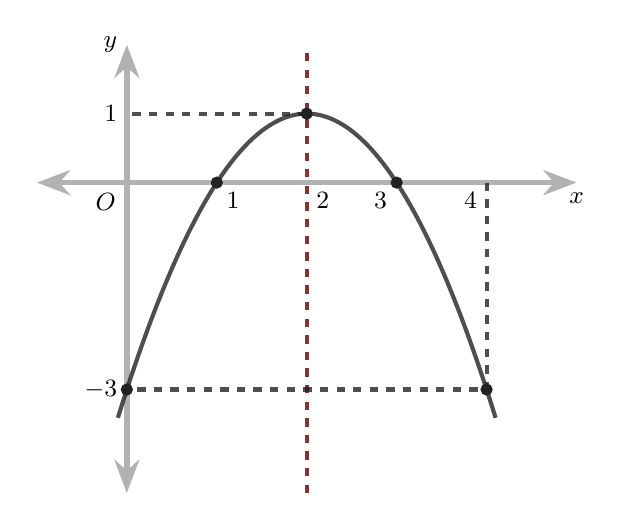
\begin{tikzpicture}
  \begin{axis}[
    font=\small\sf,
    axis lines = middle,
    axis line style={<->, line width=2pt, color=den-6!50},
    xlabel=$x$, ylabel=$y$,
    xlabel style={below, font=\small\sf},
    ylabel style={left, font=\small\sf},
    xmin=-1, xmax=5,
    ymin=-4.5, ymax=2,
    % restrict y to domain=-23:27,
    % width=12cm, height=8cm,
    xtick={},
    xticklabels={},
    xtick style={draw=none},
    ytick={1},    
    yticklabels={}, 
    ytick style={draw=none},  
    tick label style={font=\footnotesize\sf},
    clip=false,
  ]

    \node[originlabel] at (axis cs:0,0) {$O$};
    \node at (0,1) [left] {$1$};
    \node at (0,-3) [left] {$-3$};
    \node at (1,0) [below right] {$1$};
    \node at (2,0) [below right] {$2$};
    \node at (3,0) [below left] {$3$};
    \node at (4,0) [below left] {$4$};

    \addplot[domain=-.1:4.1, samples=200, line width=1.5pt, color=den-2, opacity=.8] 
        {-x^2+4*x-3};

    \addplot[dashed, line width=1.5pt, color=do-2, opacity=.8] coordinates {
        (2,-4.5)
        (2,2)
        };
    \addplot[dashed, line width=1.5pt, color=den-2, opacity=.8] coordinates {
        (2,1)
        (0,1)
        };
    \addplot[dashed, line width=1.5pt, color=den-2, opacity=.8] coordinates {
        (4,0)
        (4,-3)
        (0,-3)
        };
    \addplot[only marks, mark=*, mark size=2pt, color=den-2] coordinates {
        (0,-3)
        (1,0)
        (2,1)
        (3,0)
        (4,-3)
        };

  \end{axis}
\end{tikzpicture}

\end{document}
